\subsection{相联度对 Cache 命中率的影响}

为了进一步分析 Cache 映射方式对命中率的影响，本实验在固定 Cache 容量、块大小和替换算法的条件下，改变 Cache 的相联度，比较直接映射、组相联映射和全相联映射在同一访存序列下的 Hit/Miss 情况。

本组实验采用矩阵规模为 $N=128$ 时生成的 trace.log 作为输入，固定 Cache 块大小为 64B，替换算法为 LRU，并分别测试不同相联度下的 Cache 命中率。

\subsubsection{实验设计}

本实验固定如下参数：

\begin{itemize}
    \item Cache大小:$N = 64KB$; %Cache大小为32KB时1、2、4、8路组相联的hit rate都很小(49%左右)，full时上了95,此时不太好说明影响(如果需要可以加上)
    \item 矩阵规模:$N=128$;
    \item Cache 块大小:64B;
    \item 替换算法:LRU;
    \item 输入文件：$N=128$ 时由 NEMU 生成的 trace.log。
\end{itemize}

改变的参数为 Cache 相联度，包括：

\begin{itemize}
    \item 1 路组相联，即直接映射；
    \item 2 路组相联；
    \item 4 路组相联；
    \item 8 路组相联；
    \item 全相联映射。
\end{itemize}

其中，直接映射可以看作相联度为 1 的特殊组相联 Cache；全相联映射可以看作只有 1 个 Set、所有 Cache Line 都位于同一组内的特殊情况。

\subsubsection{实验结果}

\begin{table}[H]
\centering
\caption{相联度对 Cache 命中率的影响}
\begin{tabular}{c|c|c|c|c}
\hline
Cache 大小 & 相联度 & 映射方式 & 命中率(\%) & Miss 数 \\
\hline
64KB & 1 路 & 直接映射 & 97.83 & 92177 \\
64KB & 2 路 & 2 路组相联 & 98.16 & 78164 \\
64KB & 4 路 & 4 路组相联 & 97.26 & 116087 \\
64KB & 8 路 & 8 路组相联 & 95.46 & 192655 \\
64KB & 全相联 & 全相联映射 & 96.79 & 136480 \\
\hline
\end{tabular}
\end{table}
实验数据绘制如下柱状图:
\begin{figure}[H]
    \centering
    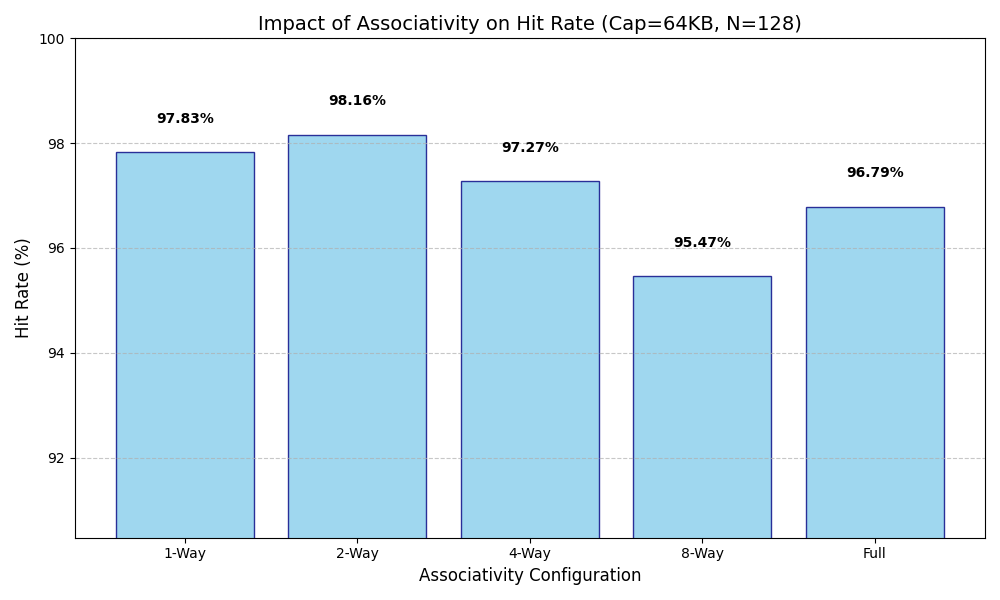
\includegraphics[width = 1\textwidth]{figure/associativity_impact.png}
    \caption{相联度对Cache命中率的影响(Cache capacity = 64KB,Cache block = 64B)}
\end{figure}

\subsubsection{实验现象与分析}

从 Cache 映射方式的角度看，相联度越高，一个主存块在 Cache 中可选择的位置越多，因而由多个活跃数据块映射到同一位置所造成的冲突缺失通常会减少。

在直接映射 Cache 中，每个主存块只能映射到唯一的 Cache Line。如果两个频繁访问的数据块恰好映射到同一行，即使 Cache 中还有其他空闲位置，也会反复发生替换，造成较多的冲突 Miss。

相比之下，组相联 Cache 允许一个主存块映射到固定 Set 内的多个 Way 中。例如 4 路组相联 Cache 中，同一个 Set 内可以同时容纳 4 个映射到该组的主存块。因此，当程序存在多个地址竞争同一组的情况时，提高相联度可以缓解冲突，提高命中率。

全相联 Cache 的冲突缺失最少，因为任意主存块都可以放入任意 Cache Line 中。但全相联映射需要在所有 Cache Line 中进行 Tag 匹配，硬件实现复杂度较高，因此在真实处理器中通常不会用于较大的 Cache，而更多用于容量较小、访问要求较高的结构，例如 TLB。

\subsubsection{实验总结}

通过本组实验可以看出，相联度主要影响 Cache 的冲突缺失。当程序的 Miss 主要来自冲突缺失时，提高相联度能够明显改善命中率；但当 Miss 主要来自冷启动缺失或容量缺失时，继续提高相联度带来的收益会逐渐减小。

因此，相联度并不是越高越好。实际 Cache 设计需要在命中率、硬件复杂度、访问延迟和功耗之间进行折中。组相联映射正是直接映射和全相联映射之间的一种折中方案。
